\indent 実験3では, 認証機構の処理能力(計算効率)を評価するための実験を行った. 
不正ノードの存在しない環境でノード数を37, 74, 112, 148, 185に設定して
250回ずつシミュレーションを行い, それぞれの実行にかかった時間を調べた.\\
\indent 実験の結果は以下の通りである. 

\begin{figure}
  \centering
  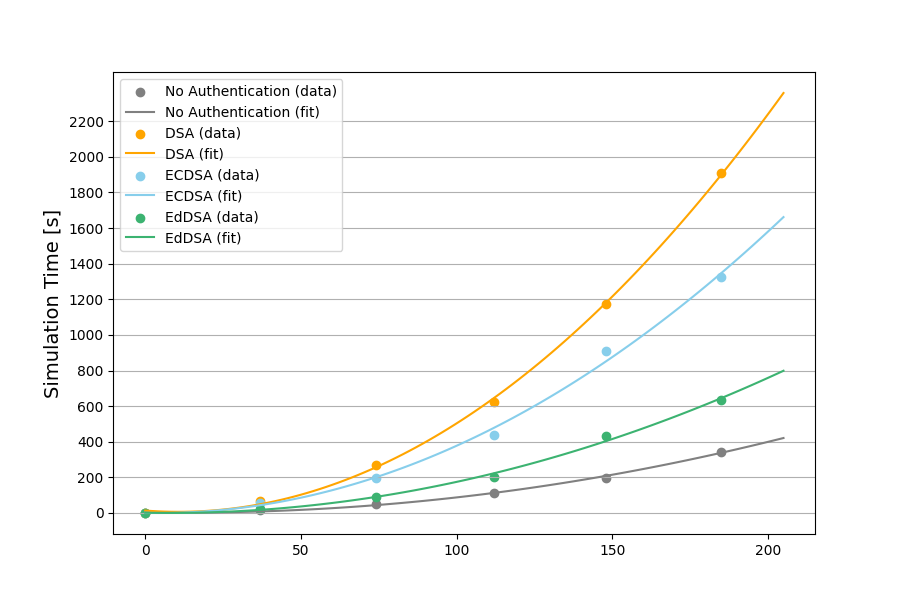
\includegraphics[width=1\textwidth]{figures/exp3_simtime.png}
  \caption{ノード数によるシミュレーション実行時間の変化}
  \label{fig:exp3_simtime}
\end{figure}
\clearpage
\setlength{\tabcolsep}{4pt}
\begin{longtable}{
    >{\raggedright\arraybackslash}p{3cm}
    >{\raggedright\arraybackslash}p{3.7cm}
    >{\raggedright\arraybackslash}p{2.5cm}
    >{\raggedright\arraybackslash}p{2.5cm}
    >{\raggedright\arraybackslash}p{2.5cm}
  }
  \caption{ノード数によるシミュレーション実行時間}
  \label{tab:exp3_simtime} \\
  \endfirsthead
  \hline
  % \multicolumn{1}{c}{Number of nodes} &
  % \multicolumn{1}{c}{No Authentication [s]} &
  % \multicolumn{1}{c}{DSA [s]} &
  % \multicolumn{1}{c}{ECDSA [s]} &
  % \multicolumn{1}{c}{Ed25519 [s]} \\ \hline \hline
  Number of nodes & No Authentication $[s]$ & DSA $[s]$ & ECDSA $[s]$ & Ed25519 $[s]$ \\ \hline \hline
  \multicolumn{1}{c}{$37$} &
  \multicolumn{1}{c}{$14.1802$} &
  \multicolumn{1}{l}{$69.9882$} &
  \multicolumn{1}{l}{$55.0108$} &
  \multicolumn{1}{l}{$24.4069$} \\
  \multicolumn{1}{c}{$74$} &
  \multicolumn{1}{c}{$50.5984$} &
  \multicolumn{1}{l}{$267.433$} &
  \multicolumn{1}{l}{$194.408$} &
  \multicolumn{1}{l}{$89.2728$} \\
  \multicolumn{1}{c}{$112$} &
  \multicolumn{1}{c}{$110.405$} &
  \multicolumn{1}{l}{$625.504$} &
  \multicolumn{1}{l}{$436.926$} &
  \multicolumn{1}{l}{$200.901$} \\
  \multicolumn{1}{c}{$148$} &
  \multicolumn{1}{c}{$196.971$} &
  \multicolumn{1}{l}{$1172.57$} &
  \multicolumn{1}{l}{$910.373$} &
  \multicolumn{1}{l}{$431.346$} \\
  \multicolumn{1}{c}{$185$} &
  \multicolumn{1}{c}{$345.059$} &
  \multicolumn{1}{l}{$1908.7$} &
  \multicolumn{1}{l}{$1324.55$} &
  \multicolumn{1}{l}{$635.155$} \\ \hline

  % $37$ & $14.1802$ & $69.9882$ & $55.0108$ & $24.4069$ \\
  % $74$ & $50.5984$ & $267.433$ & $194.408$ & $89.2728$ \\
  % $112$ & $110.405$ & $625.504$ & $436.926$ & $200.901$ \\
  % $148$ & $196.971$ & $1172.57$ & $910.373$ & $431.346$ \\
  % $185$ & $345.059$ & $1908.7$ & $1324.55$ & $635.155$ \\ \hline
\end{longtable}

\begin{longtable}{c|cc}
  \caption{1回の署名作成と署名検証にかかった時間}
  \label{tab:exp3_sigtime} \\
  \endfirsthead
  \hline
  プロトコル & 署名作成時間 $[ms]$ & 署名検証時間 $[ms]$ \\ \hline
  ECDSA & $0.371$ & $0.336$ \\
  Ed25519 & $0.031$ & $0.097$ \\ \hline
\end{longtable}

\begin{figure}
  \centering
  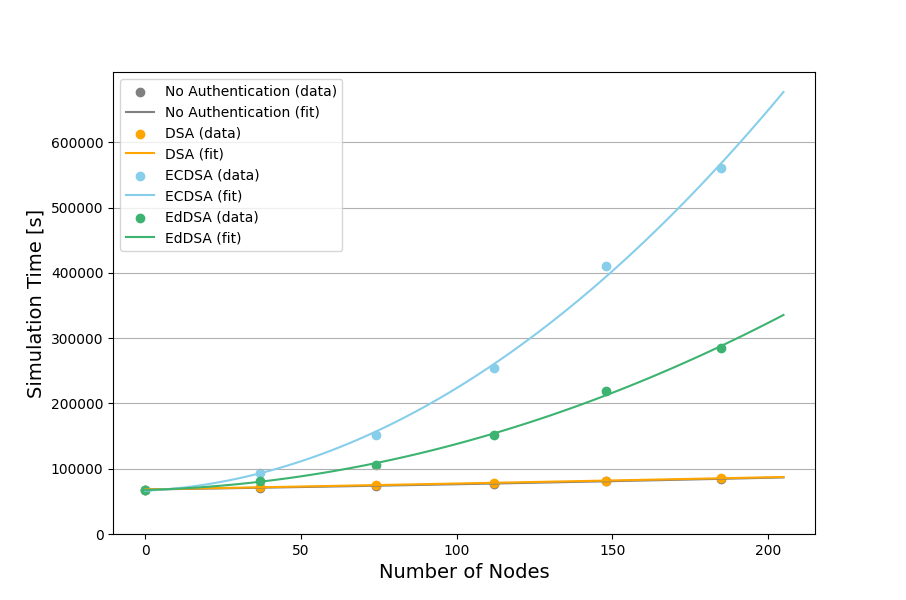
\includegraphics[width=1\textwidth]{figures/exp3_memory.png}
  \caption{ノード数によるメモリ使用量}
  \label{fig:memory_usages}
\end{figure}

\clearpage
\setlength{\tabcolsep}{4pt}
\begin{longtable}{c|cccc}
  \caption{ノード数によるメモリ使用量}
  \label{tab:exp3_memory} \\
  \endfirsthead
  \hline
  Number of nodes & No Authentication [KB] & DSA [KB] & ECDSA [KB] & Ed25519 [KB] \\ \hline \hline
  $37$ & $70939.4$ & $72023.3$ & 93749.3 & 80647.1 \\
  $74$ & 74089.7 & 74989.3 & 151853 & 106442 \\
  $112$ & 77070.1 & 78134.7 & 254247 & 151401 \\
  $148$ & 80749.9 & 81752.5 & 409965 & 219102 \\
  $185$ & 84548.1 & 85541.4 & 560753 & 285191 \\ \hline
\end{longtable}



\indent 図\ref{fig:exp3_simtime}はシミュレーションパターンごとのノード数による
実行時間の変化を近似してグラフ化したものを, 表\ref{tab:exp3_simtime}はその具体的な
値を示したものである. 表\ref{tab:exp3_sigtime}にはECDSAとEdDSAにおいて, 
1回の署名作成と署名検証にかかった時間を示した. 図\ref{fig:memory_usages}は, 
ノード数によるメモリ使用量の変化を近似してグラフ化したものを, 表\ref{tab:exp3_memory}は
その具体的な値を示したものである. \\
\indent ECDSAとEdDSAに注目して結果を評価する. 図\ref{fig:exp3_simtime}, 
表\ref{tab:exp3_sigtime}より, EdDSA, ECDSAの順番で実行時間が短く, その差は
ノード数が増加するほど大きくなっている. 言い換えると, ECDSAの実行時間の増加率が
大きいのに対し, EdDSAは比較的緩やかである. また, 表\ref{tab:exp3_sigtime}より, 
EdDSAがECDSAに比べて署名生成, 署名検証にかかる時間が短いことから, EdDSAは
ECDSAよりも計算効率が良いということが確かめられた. さらに, 
図\ref{fig:memory_usages}より, EdDSAのメモリの使用量がECDSAよりも
少なく, 実行時間と同様にECDSAの実行時間の増加率が大きいのに対し, EdDSAは比較的緩やかである. 
これらの結果から, EdDSAはECDSAと比較してネットワーク全体の計算コストの増加を抑えつつ, 
より少ないリソースで効率的に動作することが可能であり, 特に大規模なネットワーク環境において
優れたスケーラビリティを有すると考えられる. \\


